\chapter{MyDiabetes}\label{chap:syst}

Neste capítulo vamos analisar com mais detalhe a aplicação utilizada neste projeto de dissertação. A aplicação chama-se \textit{MyDiabetes} e foi desenvolvida no âmbito do mesmo projeto em que esta dissertação se insere. 

Um dos objetivos opcionais é a integração de um sistema de aconselhamento personalizado numa aplicação para registo de glicemias. Assim, e embora a aplicação, de momento, ofereça apenas a possibilidade de registo e visualização de dados, no futuro poderá ter sistema de aconselhamento. A aplicação permite também que os utilizadores enviem os seus dados, para que estes possam ser analisados. Esta é uma ferramenta importante visto que houve a necessidade de criar o nosso próprio \textit{data set}. 


\section{Objetivo da aplicação}

O objetivo desta aplicação já foi mencionado anteriormente: ajudar o doente diabético, ao oferecer uma ferramenta alternativa que permita registar e visualizar todos os parâmetros importantes, como glicose, insulina e hidratos de carbono. O \textit{smartphone} é um dispositivo bastante interessante para ter aplicações como esta: a maioria das pessoas tem um e portanto, se tiver uma aplicação pode registar a glicemia a qualquer hora e em qualquer lugar.
Além da função de registo, a aplicação permite também a visualização dos registos efetuados em forma de gráfico. Assim torna-se mais fácil detetar hiperglicemias. Ou visualizar registos de meses anteriores ou até mesmo mostrar ao médico, durante a consulta, os valores de glicemia no período entre as consultas.
Tudo isto contribui para o objetivo principal: tornar mais simples e eficaz o controlo da glicemia. 

Para este trabalho, o objetivo da aplicação foi que os utilizadores a pudessem utilizar para que se familiarizassem com uma aplicação deste tipo e também para enviar os dados necessários para análise posterior.

\section{Arquitetura}

A aplicação é bastante simples e facilmente um utilizador se habitua às suas funcionalidades. Quando um utilizador a usa pela primeira vez é necessário preencher os seus dados. Todos os dados são obrigatórios mas não são diretamente relevantes para este trabalho, como nome, data de nascimento ou altura, por exemplo. Desta forma, qualquer utilizador que quisesse enviar os seus registos para o projeto de forma anónima poderia fazê-lo, bastando para isso introduzir dados falsos. 
Por outro lado há dados que são relevantes para o cálculo da insulina, como o fator de sensibilidade. Outro tipo de dados como os limites para hipo e hiperglicemia são úteis para as futuras funcionalidades que a aplicação possa vir a ter, como a emissão de avisos, já que alguns avisos são baseados nestes valores. De notar que estes dados são registados aquando da primeira utilização, mas podem ser alterados a qualquer momento a partir do menu das definições.
A aplicação em si é constituída por um ecrã principal que tem os submenus de registo, tais como refeições, exercício, insulina, entre outros. Tem também o submenu ``Logbook'' que permite visualizar registos anteriores, através da escolha de um intervalo de tempo. Estes dados são mostrados na forma de gráfico e de lista.

A aplicação é bastante intuitiva: tem menus de registo, como registo de refeições, insulinas, exercício ou doenças. Esses registos são guardados no \textit{smartphone}, numa base de dados \textit{sqlite}. Tem também um menu para visualização dos registos efetuados, o ``Logbook''. 
No menu de definições é possível aceder a outras funcionalidades da aplicação. É possível alterar os dados, como já mencionado, mas também enviar os registos para o projeto ou gerar um relatório. Este relatório pode ser especialmente útil para mostrar ao médico na consulta pois é possível imprimi-lo e mostrar os valores de qualquer parâmetro que o utilizador queira, como glicemias por exemplo. É possível escolher, por exemplo, todas as glicemias registadas entre consultas, exportar para pdf e depois imprimir, sendo um registo limpo e de fácil leitura.


\begin{figure}[H]
    \centering
    \subfloat[Menu principal]{{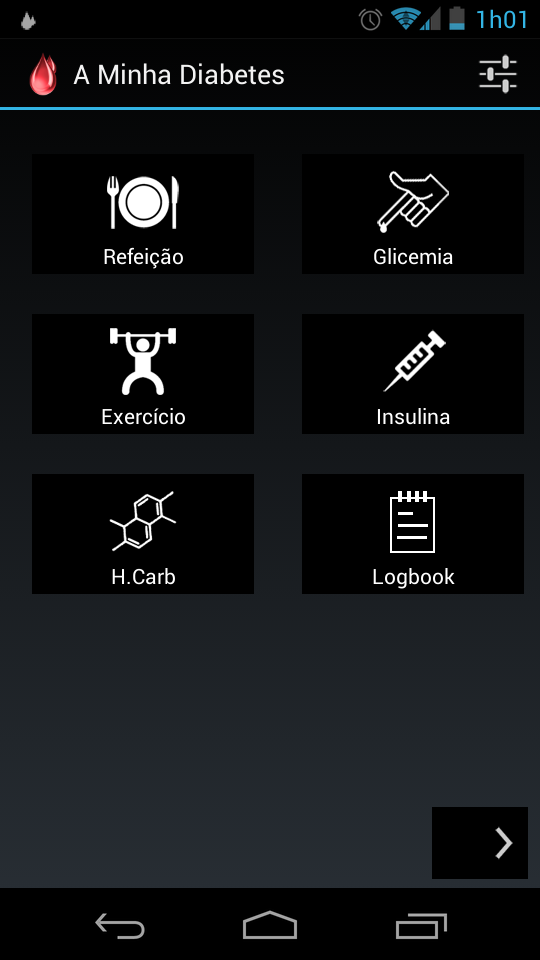
\includegraphics[width=5cm]{/home/tiago/Tese/Tese/Databases/CSV/Data/ImagensTese/mainmenu.png} }}%
    \qquad
    \subfloat[Logbook com gráfico]{{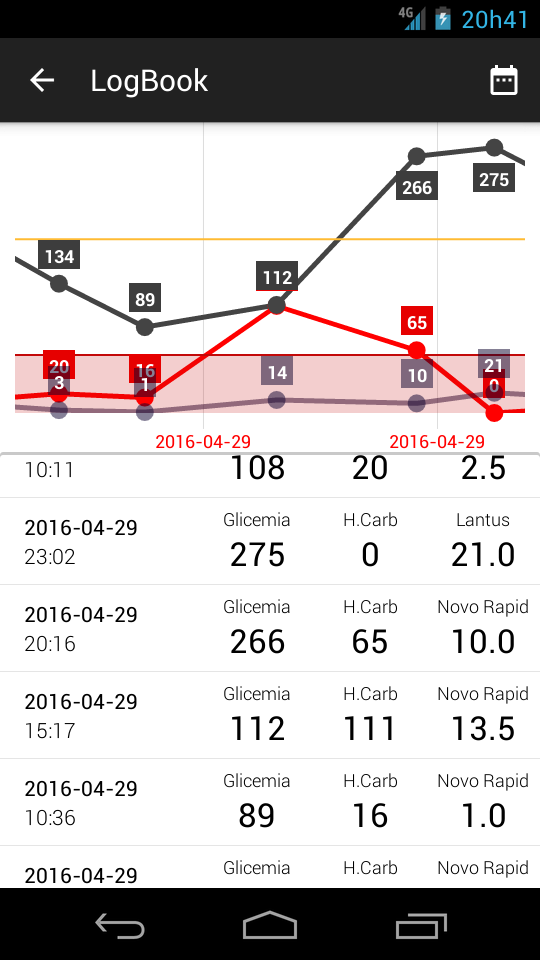
\includegraphics[width=5cm]{/home/tiago/Tese/Tese/Databases/CSV/Data/ImagensTese/logbook.png}}}%
    \caption{Algumas funcionalidades da aplicação}%
    \label{fig:example}%
\end{figure}

\section{Variáveis recolhidas}

Como já explicado anteriormente, a aplicação permite recolher qualquer tipo de dados que possa ser relevante para um bom controlo da glicemia. Além dos valores da glicose, hidratos de carbono e insulina, a aplicação permite também a recolha de outros dados, como doença e exercício, que são eventos que têm um impacto direto nos valores de glicemia. Existe também a opção de registar a \ac{HbA1c}. É possível ainda registar outros dados que, apesar de terem menos ou nenhum impacto na diabetes, podem ser indicadores do estado de saúde do utilizador e portanto permite também ter um maior controlo sobre eles, como pressão arterial, colesterol ou peso.
Sempre que é efetuado um registo, seja de que parâmetro for, a aplicação regista também o dia e hora desse mesmo registo. Saber a hora e dia de cada registo será especialmente importante para o objetivo de detetar padrões ou anomalias, ou também para análises estatísticas, uma vez que possibilitará dar uma ideia ao utilizador dos dias ou períodos do dia em que a glicemia é mais elevada. De notar que nem todos os dados registados pelos utilizadores foram recolhidos para o trabalho desta dissertação. No entanto, todos os que foram recolhidos foram usados única e exclusivamente para a análise. 

